
\documentclass[10pt,a4paper]{article}
\usepackage[margin=0.78in]{geometry}
\usepackage{booktabs,tabularx,array}
\usepackage{graphicx}
\usepackage{amsmath}
\usepackage{hyperref}
\usepackage{caption}
\usepackage{enumitem}
\usepackage{xcolor}
\usepackage{float}
\graphicspath{{figures/}}
\hypersetup{colorlinks=true,linkcolor=blue,urlcolor=blue,citecolor=blue}
\title{\textbf{Compute-Efficient Training of Small Transformer Language Models}\\
\large Investigating Training Duration, Data Quantity, and Model Capacity}
\author{SONG MINGJUN\\NUS Student ID: A034593Y}
\date{DSA4212 Final Project\\13 November 2026}
\begin{document}
\maketitle
\begin{center}
\small GitHub repository: \url{https://github.com/JS-2028/dsa4212-small-llm}
\end{center}

\begin{abstract}
Training a language model under a limited compute budget requires choices about model capacity, training duration, and data quantity. This project implements a decoder-only Transformer language model from randomly initialised weights in PyTorch and investigates these choices on TinyStories using an 8,000-token byte-pair encoding tokenizer. Three exploratory studies are reported. First, a 5.27M-parameter model's validation cross-entropy decreased from 3.976 after 500 updates to 2.511 after 5,000 updates, although the runs used different learning-rate schedules and are therefore not a fully controlled duration comparison. Second, a controlled data-scaling experiment compared 10,000, 50,000, and 100,000 stories over 5,000 updates, with three random seeds per condition. Mean validation losses were 2.5555, 2.5160, and 2.5150, respectively, suggesting a benefit from the first increase in data and little additional gain from 50,000 to 100,000 stories under this training budget. Third, under an approximately 150-second wall-clock budget, models with 5.27M, 13.82M, and 29.45M parameters achieved validation losses of 2.4671, 2.6092, and 2.8401. The smallest model performed best in this hardware- and budget-specific comparison, while larger models completed fewer updates. These results illustrate trade-offs between data diversity, optimisation progress, and model capacity. Limitations include the use of a single validation sample of fixed batches, a single seed for model scaling, no final test-set evaluation, and a small number of model configurations.
\end{abstract}

\section{Introduction}
A small language model must allocate limited computation among its parameter count, the number of optimisation updates, and the amount of training data it encounters. Increasing model size can increase representational capacity, but also raises the cost of each update. Increasing dataset size can expose a model to more diverse examples, but a fixed number of updates then covers a smaller fraction of the available corpus. Training for longer may improve predictive performance, although returns can diminish or overfitting can emerge.

This project studies these trade-offs by training a decoder-only Transformer from scratch on TinyStories. The project is motivated by compute-optimal language-model training, where model size and training-token allocation interact rather than being independent decisions \cite{hoffmann2022}. TinyStories provides a controlled domain of short, simple narratives designed to study the capabilities of small language models \cite{eldan2023}. The project asks:

\begin{quote}
\emph{How do training duration, dataset size, and model capacity affect the predictive performance of a small Transformer language model under limited computational resources?}
\end{quote}

The investigation is organised around three experiments: (E1) training duration, (E2) data quantity, and (E3) model size under a fixed wall-clock budget. The aim is not to establish universal scaling laws, but to measure the behaviour of this implementation on a Tesla T4 GPU and explain the observed trade-offs.

\section{Background}
Transformer architectures use self-attention to model dependencies between sequence positions \cite{vaswani2017}. A decoder-only language model applies causal masking so that each position predicts the next token using only preceding context. The implementation here uses learned token and positional embeddings, pre-layer normalisation, residual connections, multi-head causal self-attention, and position-wise feed-forward networks. The model is trained with next-token cross-entropy.

Byte-pair encoding (BPE) represents text as subword units and can reduce the need for a fixed word-level vocabulary \cite{sennrich2016}. Compute-optimal training research highlights the joint allocation of parameters and training tokens \cite{hoffmann2022}. Data-constrained training also raises the question of how repeated exposure and dataset diversity affect performance \cite{muennighoff2023}. These ideas motivate the project's controlled comparisons.

\section{Methods}
\subsection{Data and preprocessing}
The experiments use the public TinyStories dataset. The downloaded corpus contained 2,119,719 training stories and 21,990 validation stories. A deterministic split reserved 10,000 stories from the original training split as a held-out test set, leaving 2,109,719 training stories. The reserved test set was not used for training, tokenizer fitting, or the reported validation comparisons; due to the project deadline, no final test-set evaluation was completed.

A byte-level BPE tokenizer with an 8,000-token vocabulary was trained on a deterministic sample of 200,000 training stories only. The special tokens were \texttt{[UNK]}, \texttt{[BOS]}, \texttt{[EOS]}, and \texttt{[PAD]}. Each story was encoded and terminated with \texttt{[EOS]}. The tokenizer reconstructed the inspected sample exactly. The model's context length was 256 tokens. Training batches were sampled as contiguous windows from concatenated token streams, so a window could cross a story boundary; EOS tokens mark those boundaries.

For the initial pilot, 10,000 stories were tokenised. E2 used nested, deterministically shuffled subsets of 10,000, 50,000, and 100,000 stories. Their token counts were 2,218,441; 11,022,217; and 22,035,205, respectively. E2 and E3 used the same fixed set of 50 validation batches (batch size 32, sequence length 256) for within-experiment comparisons.

\subsection{Architecture and optimisation}
The baseline model is a decoder-only Transformer implemented in PyTorch. It uses tied token-embedding and output-projection weights, learned positional embeddings, causal multi-head attention, GELU feed-forward layers, residual connections, and pre-layer normalisation. The baseline configuration has 4 layers, embedding dimension 256, 4 attention heads, context length 256, dropout 0.1, and approximately 5.27 million trainable parameters. Larger E3 models use the same implementation with different depth and width.

Models were randomly initialised; no pretrained model weights, embeddings, or other pretrained neural components were used. Training used AdamW with betas (0.9, 0.95), weight decay 0.1, gradient clipping at 1.0, FP16 autocast and gradient scaling. The standard 5,000-update schedule used a peak learning rate of \(3\times10^{-4}\), 200 warmup updates, and cosine decay. The hardware was a Google Colab NVIDIA Tesla T4 GPU with 15.64 GB reported VRAM, using PyTorch 2.14.1+cu130.

\subsection{Evaluation}
The primary metric is mean next-token cross-entropy on fixed validation batches; lower is better. Perplexity is reported as \(\exp(\text{loss})\). Runtime and peak allocated GPU memory are secondary resource measures. E2 reports mean and sample standard deviation across three seeds. E3 is an exploratory single-seed comparison. Because all comparisons use the same tokenizer, token-level cross-entropy and perplexity are comparable within these experiments.

\section{Experiments and Results}
\subsection{E1: Training duration}
A 5.27M-parameter model trained on the initial 10,000-story pilot subset was evaluated after 500 and 5,000 updates. The 500-update run achieved validation loss 3.9758 in 28.74 seconds; the 5,000-update run achieved 2.5115 in 222.19 seconds. The latter represents a 36.8\% reduction in validation loss relative to the former.

This is exploratory evidence that additional optimisation substantially improved predictive performance in this setup. However, the two runs used different warmup lengths and cosine schedules (50 warmup updates for the 500-update pilot versus 200 for the 5,000-update run), and the validation estimates were obtained using different evaluation sampling procedures. They were not a strictly controlled experiment isolating training duration. The result should therefore be interpreted as an indicative pilot rather than a causal estimate of the effect of training time.

\subsection{E2: Training data quantity}
E2 compared nested datasets of 10,000, 50,000, and 100,000 stories. Each configuration was trained for 5,000 updates with batch size 32 and context length 256. Three seeds (1234, 2027, 2028) were run per condition. All runs used the same fixed validation batches.

\begin{table}[H]
\centering
\caption{E2 validation results across three random seeds (mean and sample standard deviation).}
\begin{tabular}{lrrrr}
\toprule
Dataset & Stories & Mean validation loss & SD & Mean perplexity\\
\midrule
D1 & 10,000 & 2.5555 & 0.0072 & 12.8777\\
D2 & 50,000 & 2.5160 & 0.0021 & 12.3786\\
D3 & 100,000 & 2.5150 & 0.0086 & 12.3672\\
\bottomrule
\end{tabular}
\end{table}

Increasing the dataset from 10,000 to 50,000 stories reduced mean validation loss by approximately 0.0395. Increasing it from 50,000 to 100,000 stories reduced mean loss by only approximately 0.0009. The standard deviations indicate that the D2--D3 difference is small relative to observed variation across seeds. The pattern is consistent with diminishing returns from additional data under a fixed 5,000-update budget, although three seeds provide limited precision and do not establish statistical significance.
\begin{figure}[H]\centering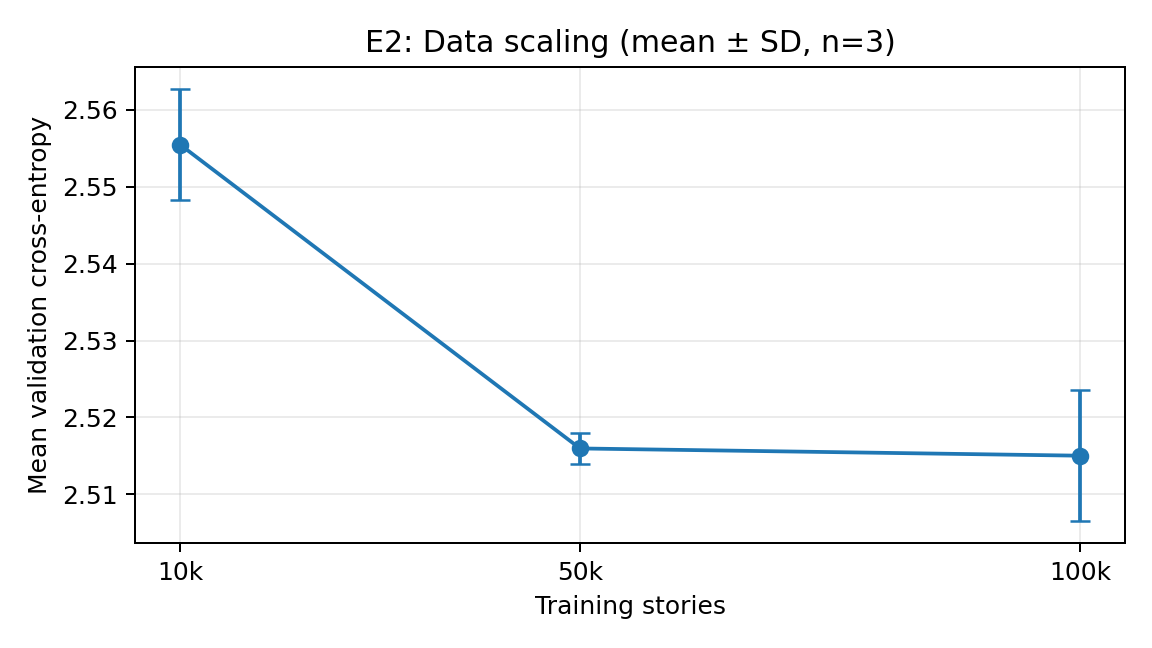
\includegraphics[width=0.78\linewidth]{e2_data_scaling.png}\caption{E2 validation loss by training-set size; error bars show sample standard deviation across three seeds.}\end{figure}

Mean training time for the replicated runs was approximately 212.3 seconds for D1, 210.8 seconds for D2, and 210.8 seconds for D3. Peak allocated GPU memory was approximately 1.44 GB across conditions. This is expected because the model and number of updates were held constant; larger datasets change the sampling pool, not the computation in each update. With a fixed update count, the larger datasets also receive fewer repeated exposures on average.

\subsection{E3: Model capacity under a fixed wall-clock budget}
E3 compared three model sizes on the 100,000-story training subset. Each model was trained for an approximately 150-second wall-clock allowance using the same batch size, context length, optimiser, and validation batches. The configurations were 4 layers/256 embedding/4 heads, 6/384/6, and 8/512/8.

\begin{table}[H]
\centering
\caption{E3 model-scaling results. Each configuration was run once.}
\begin{tabular}{lrrrrr}
\toprule
Model & Parameters & Updates & Tokens processed & Val. loss & Peak memory\\
\midrule
Small & 5.27M & 3,517 & 28.81M & 2.4671 & 1.46 GB\\
Medium & 13.82M & 1,645 & 13.48M & 2.6092 & 2.00 GB\\
Large & 29.45M & 903 & 7.40M & 2.8401 & 2.79 GB\\
\bottomrule
\end{tabular}
\end{table}

The smallest model achieved the lowest validation loss under the fixed-time comparison. As model size increased, the number of completed updates and processed tokens decreased, while peak memory increased. The result suggests that, on this T4 hardware and within this short budget, the smaller model used computation more effectively. It does not show that smaller models are generally superior: the comparison deliberately fixes elapsed time rather than updates or tokens, and each model size was tested with only one seed. The implementation also used a fixed 100-update warmup, so warmup occupied a larger fraction of the available wall-clock budget for the larger models.
\begin{figure}[H]\centering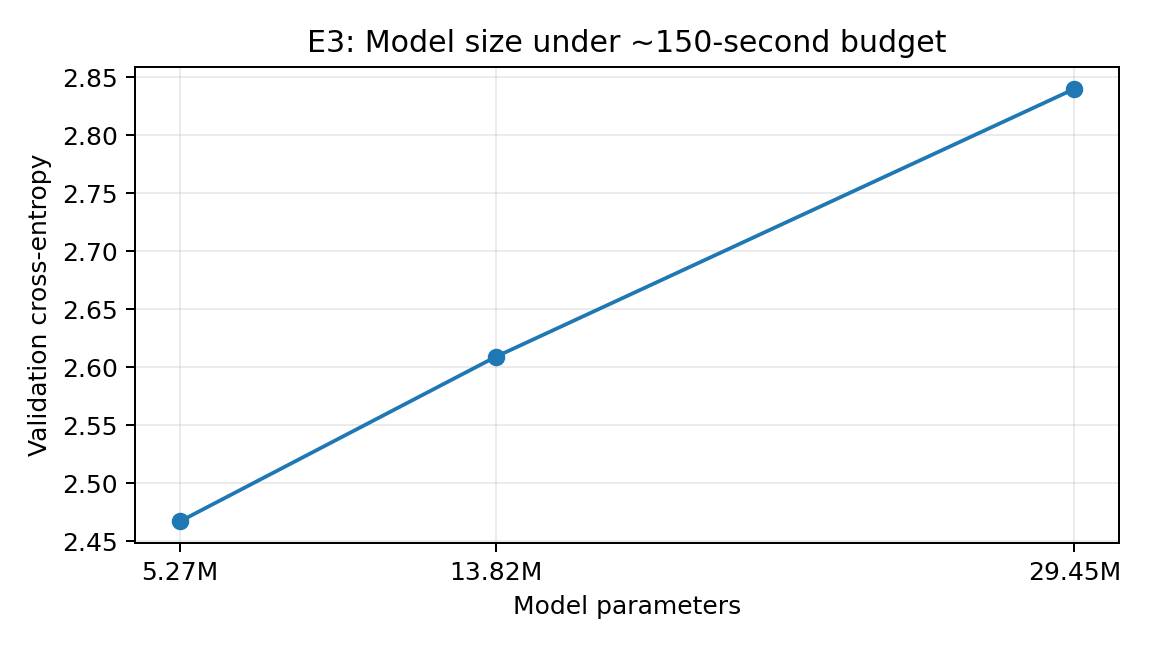
\includegraphics[width=0.78\linewidth]{e3_model_scaling.png}\caption{Validation loss against parameter count under an approximately 150-second budget.}\end{figure}

\section{Discussion}
Across the three investigations, performance depended on how the limited training budget was allocated. E1's pilot comparison showed a large improvement with substantially more updates, although schedule and evaluation differences limit causal interpretation. E2 provides the most controlled evidence: increasing data from 10,000 to 50,000 stories improved validation loss across three seeds, while the further increase to 100,000 yielded almost no additional gain under 5,000 updates. This may reflect diminishing returns, or that the fixed number of updates was insufficient to exploit the additional data.

E3 shows the cost of increasing model capacity under a wall-clock constraint. Larger models consumed more memory and completed fewer updates and token positions, and had higher validation loss. In this setting, additional capacity did not compensate for reduced optimisation progress. This finding is specific to the chosen architecture, T4 GPU, short training duration, batch size, sequence length, and learning-rate schedule.

A practical implication is that model size, data quantity, and training duration should be considered jointly. A larger corpus is not automatically useful if the model cannot see enough of it during training, and a larger model may be disadvantaged when its per-update cost sharply reduces the number of updates possible. These results are consistent with the broader motivation of compute-optimal training, but the small number of configurations and limited budget do not support fitting a scaling law.

Qualitative generations from the 5,000-update baseline contained recognisable story openings, dialogue, and moral-like endings, but also semantic contradictions, object confusion, and character inconsistency. This suggests that low validation loss alone does not guarantee coherent long-form generation. The qualitative examples were illustrative rather than scored by a blinded human evaluation, so no quantitative claim about generation quality is made.

\section{Limitations}
Several limitations qualify the findings. First, E1 was exploratory and changed the learning-rate schedule and validation sampling between runs. Second, E2 used only three seeds and one fixed set of validation batches; the standard deviations measure variation across training seeds conditional on those batches, not uncertainty over the full validation distribution. Third, E3 used one seed per model size and a short wall-clock budget, so its ranking may be sensitive to initialisation and warmup. Fourth, E3's measured elapsed time includes final evaluation overhead and can slightly exceed the nominal 150-second training-loop budget. Fifth, the reserved test split was not evaluated before submission; all reported predictive metrics are validation metrics. Sixth, only one dataset domain, tokenizer, context length, optimiser, and hardware type were investigated. Finally, the model sizes and training budgets are too limited to infer general scaling laws.

Future work should repeat E3 across multiple seeds, compare models under equal token and equal update budgets as well as equal time, evaluate on the untouched test set, test longer schedules, and investigate optimiser and context-length choices. A human or rubric-based evaluation of generated stories would complement token-level loss.

\section{Conclusion}
This project implemented and trained small decoder-only Transformer language models from random initialisation on TinyStories using a Tesla T4 GPU. The experiments indicate that longer training can improve validation performance, that increasing data from 10,000 to 50,000 stories can help under a fixed update budget while further gains diminish, and that a smaller model can outperform larger alternatives when elapsed training time is constrained. The findings are local to the experimental setup and should not be interpreted as universal prescriptions. Overall, the project demonstrates that compute-efficient language-model training involves balancing model capacity, data diversity, and optimisation progress.

\nocite{*}

\section*{AI Assistance Declaration}

Generative AI tools, including ChatGPT (OpenAI), were used
to assist with research ideation, experimental planning,
PyTorch implementation, code debugging, interpretation of
experimental results, and editing and drafting of the report.
All experiments were executed by the author using Google
Colab and an NVIDIA Tesla T4 GPU. The author is responsible
for reviewing and verifying the implementation, experimental
results, references, and final submitted work, and for ensuring
an understanding of the methods and conclusions presented.

\bibliographystyle{plain}
\bibliography{references}
\end{document}
